\documentclass[a4paper,12pt]{article}
\usepackage{amsmath, amssymb}
\usepackage{dsfont}
\usepackage{tikz} 
\usepackage[utf8]{inputenc}
%\usepackage[spanish]{babel}
\usepackage{amsmath}
\usepackage{amsfonts}
\usepackage{amssymb}
\usepackage{graphicx}
\usepackage{exercise}

\author{Pilar Barbero Iriarte}

\newenvironment{exercise}[1]% environment name
{% begin code
  \par\vspace{\baselineskip}\noindent
  \textbf{Ejercicio (#1)}\begin{itshape}%
  \par\vspace{\baselineskip}\noindent\ignorespaces
}%
{% end code
  \end{itshape}\ignorespacesafterend
}




\begin{document}

\begin{titlepage}
\begin{center}


% Upper part of the page. The '~' is needed because \\
% only works if a paragraph has started.

\textsc{\LARGE M\'aster en Modelizaci\'on \\e Investigaci\'on Matem\'atica,\\ Estad\'istica y Computaci\'on }\\[1.5cm]
{\large \today}

\textsc{Ejercicios Primera Parte}\\[0.5cm]

% Title
\vfill

{ \huge \bfseries Modelos de Log\'istica \\[0.4cm] }

\vfill



% Author and supervisor
\noindent
\begin{minipage}{0.4\textwidth}
\begin{flushleft} \large

\includegraphics[width=1.1\textwidth]{../logoUZ.png}~\\[1cm]
\emph{Autor:}\\
Pilar Barbero Iriarte 
\end{flushleft}
\end{minipage}%
\begin{minipage}{0.4\textwidth}
\begin{flushright} \large

\includegraphics[width=0.85\textwidth]{../logoULL.png}~\\[1cm]
\emph{Profesor:} \\
Antonio Sede\~no Noda
\end{flushright}
\end{minipage}

% Bottom of the page
\end{center}


\end{titlepage}

\pagebreak
\tableofcontents
\pagebreak

\section{Modelizaci\'on}

\begin{exercise}{1}
Un fabricante de tecnolog\'ia solar considera producir masa de m\'odulo de celda (producto 1, $x_1$) para sat\'elites de aplicaci\'on atmosf\'erica  y m\'odulo de celda de astilla (producto 2, $x_2$) para uso de calculadoras de bolsillo. Se conoce una lista donde las ventas son estimadas entre $5$ y $12$ unidades para los productos $1$ y $2$, respectivamente, como pron\'ostico del dpto. de marketing.

El presidente de la empresa ha establecido las siguiente meta para esta particular operaci\'on de producci\'on para el siguiente mes:

Tener un beneficio de al menos 33 unidades, es decir, $x_1 + 3x_2 \geq 33$\\
Objetivo: Limitar el l\'imite de roturas a 36, es decir, $3x_1 + 2x_2 \leq 36$\\
Las restricciones asociadas al proceso de producci\'on son:\\

\begin{itemize}

\item Capacidad de la m\'aquina: $0.5x_1 + 0.25x_2 \leq 8$

\item Capacidad de ensamblado: $0.2x_1 + 0.2x_2 \leq 4$

\item Materiales bruto: $x_1 + 5x_2 \leq 72$

\end{itemize}
\end{exercise}


Modelamos de la siguiente forma:


\begin{itemize}

\item[\textbf{Variables}]
	\begin{itemize}
		\item[] $0 \leq x_1 \leq 5 \text{ con } x_1\in \mathds{Z}$
		\item[] $0 \leq x_2 \leq 12 \text{ con } x_2\in \mathds{Z}$
	\end{itemize}
	
\item[\textbf{Restricciones}]

\begin{itemize}

		\item[] $3x_1 + 2x_2 \leq 36$
		\item[] $0.5x_1 + 0.25x_2 \leq 8$
		\item[] $0.2x_1 + 0.2x_2 \leq 4$
		\item[] $x_1 + 5x_2 \leq 72$
		\item[] $x_1 + 3x_2 \geq 33$
\end{itemize}
	
	
\item[\textbf{Funci\'on Objetivo}]
	\begin{itemize}
			\item[] $\text{m\'in}\,z = 33 - x_1 - 3x_2$
	\end{itemize}
\end{itemize}

\pagebreak

\section{Interpretaci\'on}
Se ha utilizado Microsoft Solver Foundation con el fin de resolver el problema anteriormente modelizado. 

El modelo consta de dos variables $x_1$ y $x_2$ que introducimos en el apartado de \textit{Decisions} definidas en el rango previamente descrito y asign\'andoles la cualidad de \textit{Integer}.

Las $5$ restricciones previamente definidas se han an\~adido al MSF en el apartado de \textit{Constraints}.

\begin{itemize}
\item[c1:] $3*x1 + 2*x2 <= 36$
\item[c2:] $0.5x1 + 0.25x2 <= 8$
\item[c3:] $0.2*x1 + 0.2*x2 <= 4$
\item[c4:] $x1 + 5*x2 <= 72$
\item[c5:] $x1 + 3*x2 >= 33$
\end{itemize}

Si las dibujamos en el eje cartesiano, podemos empezar a intuir la regi\'on en la que va a estar nuestra soluci\'on,

\begin{figure}[h]
  \centering
	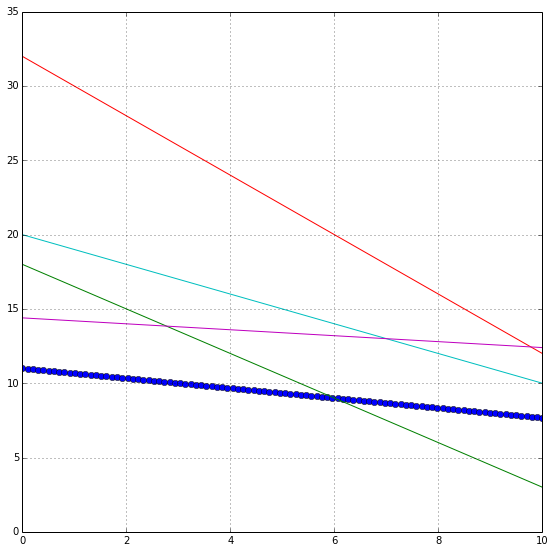
\includegraphics[scale=0.4]{constraints.png}
	  \caption{Constraints}
\end{figure}

Todas las inecuaciones, excepto la representada en azul con trazos m\'as gruesos definen la parte del plano por debajo de su funci\'on correspondiente. La funci\'on representada en azul con trazos m\'as gruesos se corresponde a la inecuaci\'on \textit{c1} y est\'a define la parte superior del plano.\\

El \'area del primer cuadrante resaltada es el \'area que nos define nuestras restricciones.
\begin{figure}[h]
  \centering
	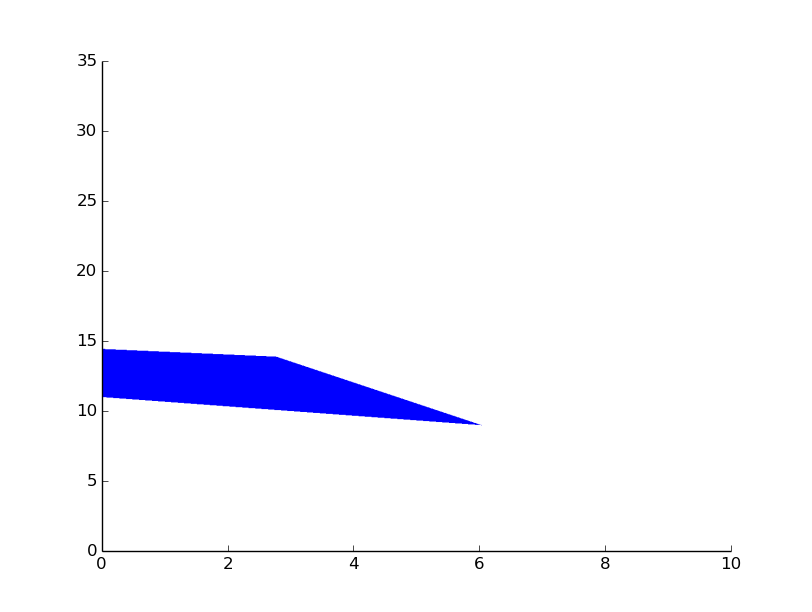
\includegraphics[scale=0.5]{constraints_area.png}
	  \caption{Constraints}
\end{figure}


Posteriormente se ha an\~adido la funci\'on objetivo a minimizar en el apartado \textit{Goals}: $$33 - x_1 -3*x_2$$

Se ha \textit{checkeado} la sintaxis del modelo y se ha resuelto el problema. Se obtiene la siguiente tabla:\\

\begin{figure}[h]
  \centering
	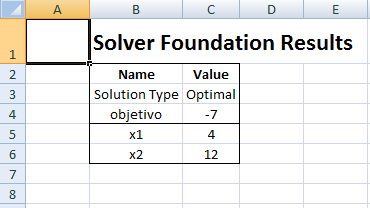
\includegraphics[scale=0.7]{msf.png}
	  \caption{Resultado MSF}
\end{figure}

Es f\'acil ver que los datos de la salida cumplen la funci\'on objetivo,

$$ -7 = \text{min }z = 33 - x_1 - 3x_2 = 33 - 4 - 3 \cdot 12$$

Ahora bien, ¿c\'omo interpretamos esta salida? Los resultados de las decisiones $x_1$ y $x_2$ son claros, $x_1$ debe valer $4$ y $x_2$ debe valer $12$. Utilizando esto en la ecuaci\'on que nos genera el beneficio nos encontrar\'iamos con el beneficio siguiente,

$$ x_1 + 3x_2 = 4 + 3 \cdot 12 = 40 \text{ unidades de beneficio}$$ 

\end{document}